% mnras_template.tex
%
% LaTeX template for creating an MNRAS paper
%
% v3.2 released 20 July 2023
% (version numbers match those of mnras.cls)
%
% Copyright (C) Royal Astronomical Society 2015
% Authors:
% Keith T. Smith (Royal Astronomical Society)

\documentclass[fleqn,usenatbib]{mnras}

\usepackage{newtxtext,newtxmath}
\usepackage{graphicx}
\usepackage{booktabs}
\usepackage{amsmath}
\usepackage{multirow}
\usepackage{xspace}

% Only include extra packages you actually need

%%%%%%%%%%%%%%%%%%%%%%%%%%%%%%%%%%%%%%%%%%%%%%%%%%

%%%%% AUTHORS - PLACE YOUR OWN COMMANDS HERE %%%%%

\newcommand{\feh}{$\mathrm{[Fe/H]}$\xspace}
\newcommand{\mgfe}{$\mathrm{[Mg/Fe]}$\xspace}
\newcommand{\sife}{$\mathrm{[Si/Fe]}$\xspace}
\newcommand{\alfe}{$\mathrm{[Al/Fe]}$\xspace}
\newcommand{\bafe}{$\mathrm{[Ba/Fe]}$\xspace}
\newcommand{\cefe}{$\mathrm{[Ce/Fe]}$\xspace}
\newcommand{\eufe}{$\mathrm{[Eu/Fe]}$\xspace}
\newcommand{\cfe}{$\mathrm{[C/Fe]}$\xspace}
\newcommand{\ofe}{$\mathrm{[O/Fe]}$\xspace}
\newcommand{\co}{C/O\xspace}
\newcommand{\kms}{km~s$^{-1}$\xspace}

%%%%%%%%%%%%%%%%%%%%%%%%%%%%%%%%%%%%%%%%%%%%%%%%%%

%%%%%%%%%%%%%%%%%%% TITLE PAGE %%%%%%%%%%%%%%%%%%%

\title[Chemical Memory of the Milky Way]{The Chemical Memory of the Milky Way: Permanent Multi-Element Fingerprints in Open Clusters and Their Dissolved Field Star Populations}

\author[D. Certan]{David Certan$^{1}$\thanks{E-mail: david@certan.xyz}\\
$^{1}$Independent Researcher}

\date{Accepted XXX. Received XXX; in original form XXX}

\pubyear{2025}

\begin{document}
\label{firstpage}
\pagerange{\pageref{firstpage}--\pageref{lastpage}}
\maketitle

\begin{abstract}
Stars form in clusters from molecular clouds with distinct chemistry, but tracing origins after dissolution remains central to Galactic archaeology.
We present 15 empirical tests of multi-element chemical fingerprints using GALAH DR4 (917\,588 stars, 655 clusters) and APOGEE DR17 (OCCAM VAC; 2515 stars, 85 clusters).
Open clusters carry distinct fingerprints confirmed independently in both surveys (Kruskal--Wallis $p < 10^{-10}$).
Coherence is spatially independent (Mantel $r = -0.010$, $p = 0.60$), satisfying a necessary condition for chemical tagging.
The fingerprint spans multiple nucleosynthetic channels: alpha-element scatter is $2\times$ tighter than s-process scatter in 98.1 per cent of 592 clusters (Wilcoxon $p = 1.8 \times 10^{-98}$), reflecting core-collapse versus AGB enrichment timescales.
Using fixed-threshold 4D matching of 253 cluster templates against 519\,547 field stars, we recover dissolved members at ${\sim}3\times$ enrichment, confirmed by barium proximity ($p = 3.6 \times 10^{-41}$) and kinematic coherence ($p = 3.7 \times 10^{-37}$).
The permanence test reveals no decay over 0--10~Gyr (Spearman $\rho = +0.097$, $p = 0.14$; $\tau = 100 \pm 280$~Gyr; AIC favours flat model by $\Delta\mathrm{AIC} = 2.8$), consistent with permanent chemical identity, ruling out decay shorter than ${\sim}5$~Gyr at $2\sigma$.
Coherence decreases toward the inner disc ($\rho = -0.228$, $p = 3.4 \times 10^{-9}$).
Individual recovery at 0.05~dex precision requires age as a sixth dimension; 0.02~dex surveys with asteroseismic ages will enable routine recovery.
\end{abstract}

\begin{keywords}
stars: abundances -- open clusters and associations: general -- Galaxy: disc -- Galaxy: stellar content -- methods: statistical
\end{keywords}

%%%%%%%%%%%%%%%%%%%%%%%%%%%%%%%%%%%%%%%%%%%%%%%%%%

%%%%%%%%%%%%%%%%% BODY OF PAPER %%%%%%%%%%%%%%%%%%

\section{Introduction}
\label{sec:intro}

Stars form in clusters and associations from giant molecular clouds whose chemical composition reflects the integrated nucleosynthetic history of the local interstellar medium (ISM).
Because individual molecular clouds occupy distinct locations in the Galaxy and sample different enrichment histories, the stars born from a given cloud inherit a chemical composition that can differ measurably from those of other birth sites.
This chemical identity is imprinted at formation and, for elements that are not altered by internal stellar processes, should persist for the lifetime of the star.

Most open clusters dissolve within a few hundred Myr due to tidal interactions with the Galactic disc, giant molecular clouds, and spiral arms \citep{BinneyTremaine2008, Meingast2019}.
Their former members disperse into the general field population, losing spatial and kinematic coherence on timescales of order 1~Gyr.
Tracing the birth origins of these dissolved stars is the central challenge of Galactic archaeology.

\citet{Freeman2002} proposed the concept of \emph{chemical tagging}: identifying stellar birth siblings purely through their shared abundance patterns.
If birth clusters possess unique multi-element chemical signatures, and if these signatures survive the dissolution process, then the formation history of the Galaxy is permanently encoded in the chemical abundances of its living stars.

Early observational support came from \citet{DeSilva2006, DeSilva2007}, who demonstrated that stars in the HR~1614 moving group and the Hyades share chemical abundances at the 0.03~dex level across multiple elements, consistent with a common origin.
\citet{BlandHawthorn2010} developed the theoretical framework, predicting that chemical tagging requires measurements of ${\sim}10$ abundance dimensions at precisions of ${\sim}0.03$~dex to uniquely identify birth clusters among ${\sim}10^5$ formation events.
\citet{Ting2015} explored the dimensionality requirements quantitatively, finding that the effective chemical dimensionality of stellar populations is limited by correlations among elements.
\citet{Hogg2016} demonstrated that chemical tagging could identify phase-space structures in APOGEE data, establishing proof of concept.

Despite this progress, several fundamental questions remain open.
First, does the chemical fingerprint persist across Gyr timescales, or does it degrade through processes such as radial migration, stellar evolution, or measurement systematics?
Second, can the fingerprint be recovered at the population level in the dissolved field star population, and if so, with what statistical significance?
Third, does the fingerprint have internal structure that reflects the nucleosynthetic processes responsible for different element groups?

This paper addresses these questions through a systematic series of 15 empirical tests using two independent spectroscopic surveys: GALAH DR4 \citep{Buder2024}, comprising 917\,588 stars with abundances for up to 30 elements, and APOGEE DR17 \citep{Abdurrouf2022} with the OCCAM membership catalogue \citep{Donor2020}, providing 2515 stars in 85 clusters with high-resolution $H$-band spectroscopy.
We test the reality, spatial independence, multi-element structure, nucleosynthetic hierarchy, field star recoverability, permanence, and Galactic environmental dependence of the chemical fingerprint.

The paper is organized as follows.
Section~\ref{sec:data} describes the survey data and quality cuts.
Section~\ref{sec:methods} defines the statistical methods.
Section~\ref{sec:results} presents the results of the 15-test series.
Section~\ref{sec:pipeline} describes the individual star recovery pipeline applied to three test clusters.
Section~\ref{sec:discussion} discusses the implications for Galactic archaeology.
Section~\ref{sec:conclusions} summarizes the conclusions.


\section{Data}
\label{sec:data}

\subsection{GALAH DR4}
\label{sec:galah}

We use the fourth data release of the Galactic Archaeology with HERMES survey \citep[GALAH DR4;][]{Buder2024}, which provides stellar parameters and chemical abundances for 917\,588 stars observed with the HERMES multi-object spectrograph on the Anglo-Australian Telescope.
HERMES operates at a resolving power of $R \sim 28\,000$ across four CCD channels covering 4713--7887~\AA, enabling measurements of up to 30 elemental abundances per star.

We apply the following quality cuts: signal-to-noise ratio $\mathrm{SNR} > 30$, \texttt{flag\_sp} $= 0$ (indicating no problems with the stellar parameter determination), and valid unflagged abundances in the chemical dimensions used for each test.
After these cuts, 214\,104 stars remain with valid \co ratios.

The \co ratio is computed from the individual carbon and oxygen abundances as $\mathrm{C/O} = 10^{\mathrm{[C/Fe]}} / 10^{\mathrm{[O/Fe]}}$, providing a dimensionless ratio that is insensitive to the overall metallicity scale.

\subsection{APOGEE DR17 OCCAM VAC}
\label{sec:apogee}

As an independent validation dataset, we use the Apache Point Observatory Galactic Evolution Experiment \citep[APOGEE;][]{Abdurrouf2022} seventeenth data release, which provides high-resolution ($R \sim 22\,500$) $H$-band spectra.
Cluster membership is assigned using the Open Cluster Chemical Abundances and Mapping \citep[OCCAM;][]{Donor2020} value-added catalogue, which provides probability-based membership for stars in known open clusters.

After quality cuts (SNR $> 50$, \texttt{STAR\_BAD} flag excluded), we retain 2515 stars in 85 clusters.
The APOGEE dataset provides an independent check on all results derived from GALAH, as the two surveys use different spectrographs, wavelength ranges, reduction pipelines, and abundance determination methods.

\subsection{Cluster ages}
\label{sec:ages}

Cluster ages are drawn from \citet{CantatGaudin2020}, who performed isochrone fitting to Gaia photometry for 2017 open clusters.
Ages are reported as $\log(\mathrm{age})$ and converted to linear age in Gyr.
We match these to both GALAH and APOGEE clusters by normalized name matching, obtaining ages for 606 of 655 GALAH clusters and 81 of 85 APOGEE clusters.
The age range spans 0.002--6.3~Gyr.

\subsection{Field star sample}
\label{sec:field}

For the dissolved cluster recovery tests (Section~\ref{sec:recovery}), we construct a field star sample by excluding all GALAH stars within $0.5\degr$ of any known cluster centre from the \citet{CantatGaudin2020} catalogue.
After quality cuts and cluster exclusion, the field star sample comprises 519\,547 stars.
This sample represents the dissolved population search space in which we seek chemical siblings of known clusters.


\section{Methods}
\label{sec:methods}

\subsection{Chemical Coherence Ratio}
\label{sec:ccr}

We define the Chemical Coherence Ratio (CCR) as the ratio of the between-cluster \co scatter to the within-cluster \co scatter:
\begin{equation}
\mathrm{CCR} = \frac{\sigma_{\mathrm{between}}}{\sigma_{\mathrm{within}}} \,,
\label{eq:ccr}
\end{equation}
where $\sigma_{\mathrm{between}}$ is the standard deviation of cluster-mean \co values across all clusters, and $\sigma_{\mathrm{within}}$ is the median of the per-cluster \co standard deviations.
A CCR significantly greater than unity indicates that clusters are chemically distinct: the inter-cluster variation exceeds the intra-cluster variation.

The statistical significance of inter-cluster chemical differences is assessed with the Kruskal--Wallis test \citep{Kruskal1952}, a non-parametric one-way analysis of variance that tests whether multiple groups are drawn from the same distribution.

\subsection{Multi-element coherence}
\label{sec:multielement}

For each cluster, we compute the intra-cluster scatter (standard deviation) in \co, \mgfe, \sife, \alfe, and \feh.
A cluster is classified as ``coherent'' in a given element if its internal scatter falls below a threshold set by the typical measurement precision: 0.05~dex for \co, \mgfe, and \sife; 0.05~dex for \alfe; and 0.05~dex for \feh.
The correlation structure among scatter values across elements is quantified using Spearman rank correlations.
The association between coherence in different elements is tested using Fisher's exact test on $2 \times 2$ contingency tables.

\subsection{Field star matching}
\label{sec:matching}

We employ fixed-threshold matching: a field star is classified as a chemical match to a cluster template if it falls within $\pm \delta$ of the cluster centroid in all $N$ chemical dimensions simultaneously.
The matching thresholds are: \co $\pm 0.08$, \mgfe $\pm 0.05$, \sife $\pm 0.05$, and \feh $\pm 0.10$~dex.
These thresholds are chosen to be ${\sim}2\times$ the typical intra-cluster scatter, balancing completeness against contamination.

\subsection{Enrichment factor}
\label{sec:enrichment}

For each cluster template, we count the number of observed field star matches $N_{\mathrm{obs}}$.
We then generate a null distribution by centring the same matching hypercube on 200 randomly selected field stars and counting matches at each random location.
The enrichment factor is defined as:
\begin{equation}
E = \frac{N_{\mathrm{obs}}}{\mathrm{median}(N_{\mathrm{null}})} \,.
\label{eq:enrichment}
\end{equation}
The $p$-value is computed as the fraction of null iterations in which $N_{\mathrm{null}} \geq N_{\mathrm{obs}}$.
An enrichment $E > 1$ indicates an excess of chemical matches around the cluster template relative to random field locations.

\subsection{Alpha-weighted Mahalanobis distance}
\label{sec:mahalanobis}

For covariance-based matching, we weight chemical dimensions according to their discriminating power as determined by the nucleosynthetic hierarchy (Section~\ref{sec:nucleosynthetic}).
Alpha-process elements (\mgfe and \sife) receive double weight, the \co ratio receives standard weight, and \feh receives half weight.
The weighted Mahalanobis distance is:
\begin{equation}
D_M^2 = \sum_i w_i \frac{(x_i - \mu_i)^2}{\sigma_i^2} \,,
\label{eq:mahalanobis}
\end{equation}
where $x_i$ is the field star abundance, $\mu_i$ is the cluster centroid, $\sigma_i$ is the cluster scatter, and $w_i$ is the dimension weight.

\subsection{Mantel test}
\label{sec:mantel}

The Mantel test \citep{Mantel1967} assesses whether the chemical distance matrix between clusters is correlated with their spatial distance matrix.
The Mantel statistic $r$ is the Pearson correlation between the upper triangles of the two distance matrices.
Statistical significance is evaluated against 10\,000 permutations of the cluster labels.
A non-significant Mantel statistic indicates that chemically similar clusters are not preferentially spatial neighbours, satisfying a necessary condition for chemical tagging.


\section{Results}
\label{sec:results}

\subsection{Chemical fingerprints are real and instrument-independent}
\label{sec:reality}

We first test whether open clusters carry chemically distinct \co distributions.
In the GALAH dataset, we analyse 655 clusters with $\geq 3$ members each.
The Kruskal--Wallis test yields $p < 10^{-10}$, demonstrating that the inter-cluster \co variation far exceeds what would be expected if all clusters were drawn from the same parent distribution.

Independently, the APOGEE OCCAM dataset yields a Kruskal--Wallis statistic for \co across 85 clusters with $p = 8.8 \times 10^{-104}$, confirming the result with a completely independent instrument, wavelength range, and analysis pipeline.

Among the 85 APOGEE clusters, 41 (48 per cent) have intra-cluster \co scatter below 0.05~dex, which we classify as ``coherent.''
Table~\ref{tab:coherent_clusters} lists the 15 most multi-element-coherent clusters from the APOGEE analysis.

\begin{table}
\centering
\caption{Top 15 most multi-element-coherent APOGEE clusters, ranked by composite coherence score (sum of scatter across five abundance dimensions). CCT indicates whether the cluster satisfies the C/O coherence threshold ($\sigma < 0.05$~dex).}
\label{tab:coherent_clusters}
\begin{tabular}{lcccccc}
\toprule
Cluster & Score & $\sigma_{\mathrm{C/O}}$ & $\sigma_{\mathrm{Mg}}$ & $\sigma_{\mathrm{Si}}$ & $\sigma_{\mathrm{Al}}$ & $\sigma_{\mathrm{Fe}}$ \\
\midrule
NGC 2447    & 0.051 & 0.033 & 0.002 & 0.007 & 0.017 & 0.013 \\
NGC 6866    & 0.089 & 0.038 & 0.017 & 0.005 & 0.021 & 0.016 \\
FSR 0394    & 0.093 & 0.029 & 0.002 & 0.019 & 0.037 & 0.016 \\
Berkeley 98 & 0.097 & 0.032 & 0.021 & 0.008 & 0.016 & 0.016 \\
NGC 1907    & 0.103 & 0.059 & 0.008 & 0.014 & 0.032 & 0.007 \\
Berkeley 75 & 0.114 & 0.050 & 0.015 & 0.015 & 0.014 & 0.017 \\
Czernik 20  & 0.115 & 0.053 & 0.017 & 0.016 & 0.014 & 0.011 \\
IC 1369     & 0.117 & 0.030 & 0.011 & 0.008 & 0.037 & 0.039 \\
Czernik 21  & 0.118 & 0.035 & 0.019 & 0.020 & 0.025 & 0.008 \\
NGC 1193    & 0.121 & 0.024 & 0.014 & 0.003 & 0.095 & 0.018 \\
Trumpler 20 & 0.124 & 0.041 & 0.014 & 0.014 & 0.033 & 0.022 \\
King 5      & 0.131 & 0.045 & 0.003 & 0.022 & 0.046 & 0.024 \\
Berkeley 17 & 0.139 & 0.028 & 0.018 & 0.015 & 0.036 & 0.032 \\
NGC 2324    & 0.141 & 0.077 & 0.010 & 0.013 & 0.039 & 0.020 \\
Trumpler 5  & 0.142 & 0.028 & 0.029 & 0.012 & 0.048 & 0.015 \\
\bottomrule
\end{tabular}
\end{table}


\subsection{Chemical order is spatially independent}
\label{sec:spatial}

A necessary condition for chemical tagging is that chemically similar clusters are not simply spatial neighbours.
If chemical similarity merely traced local ISM homogeneity, the chemical tag would be degenerate with spatial position and would not provide independent birth-site information.

The Mantel test on the 655 GALAH clusters yields $r = -0.010$ with $p = 0.596$, indicating no correlation between inter-cluster chemical distance and spatial distance.
When controlling for age via partial correlation, the result is unchanged ($r_{\mathrm{partial}} = -0.009$).
Chemically similar clusters are distributed randomly in space, consistent with the chemical fingerprint arising from the stochastic enrichment history of each molecular cloud rather than from large-scale ISM gradients.

\subsection{Multi-element fingerprint structure}
\label{sec:multielement_results}

Among the 39 \co-coherent APOGEE clusters (with $\sigma_{\mathrm{C/O}} < 0.05$~dex), 31 (79 per cent) are also coherent in \mgfe, 27 (69 per cent) in \sife, 28 (72 per cent) in \alfe, and 24 (62 per cent) in \feh.
Eighteen clusters (46 per cent) are simultaneously coherent in all four additional elements.

Fisher's exact test for the association between \co and \mgfe coherence yields an odds ratio of 4.69 ($p = 2.7 \times 10^{-3}$), indicating that coherence in one element is significantly associated with coherence in another.
The mean Spearman $\rho$ across all 10 pairs of scatter values is $+0.483$, with all individual correlations significant at $p < 10^{-3}$.
The strongest correlations are \mgfe versus \sife ($\rho = +0.684$, $p = 1.9 \times 10^{-12}$) and \co versus \mgfe ($\rho = +0.576$, $p = 1.9 \times 10^{-8}$).

This result demonstrates that the chemical fingerprint is not a single-element phenomenon but a correlated multi-dimensional structure: clusters that are tight in one abundance ratio tend to be tight in all.
Fig.~\ref{fig:multielement} illustrates the multi-element coherence matrix.

\begin{figure}
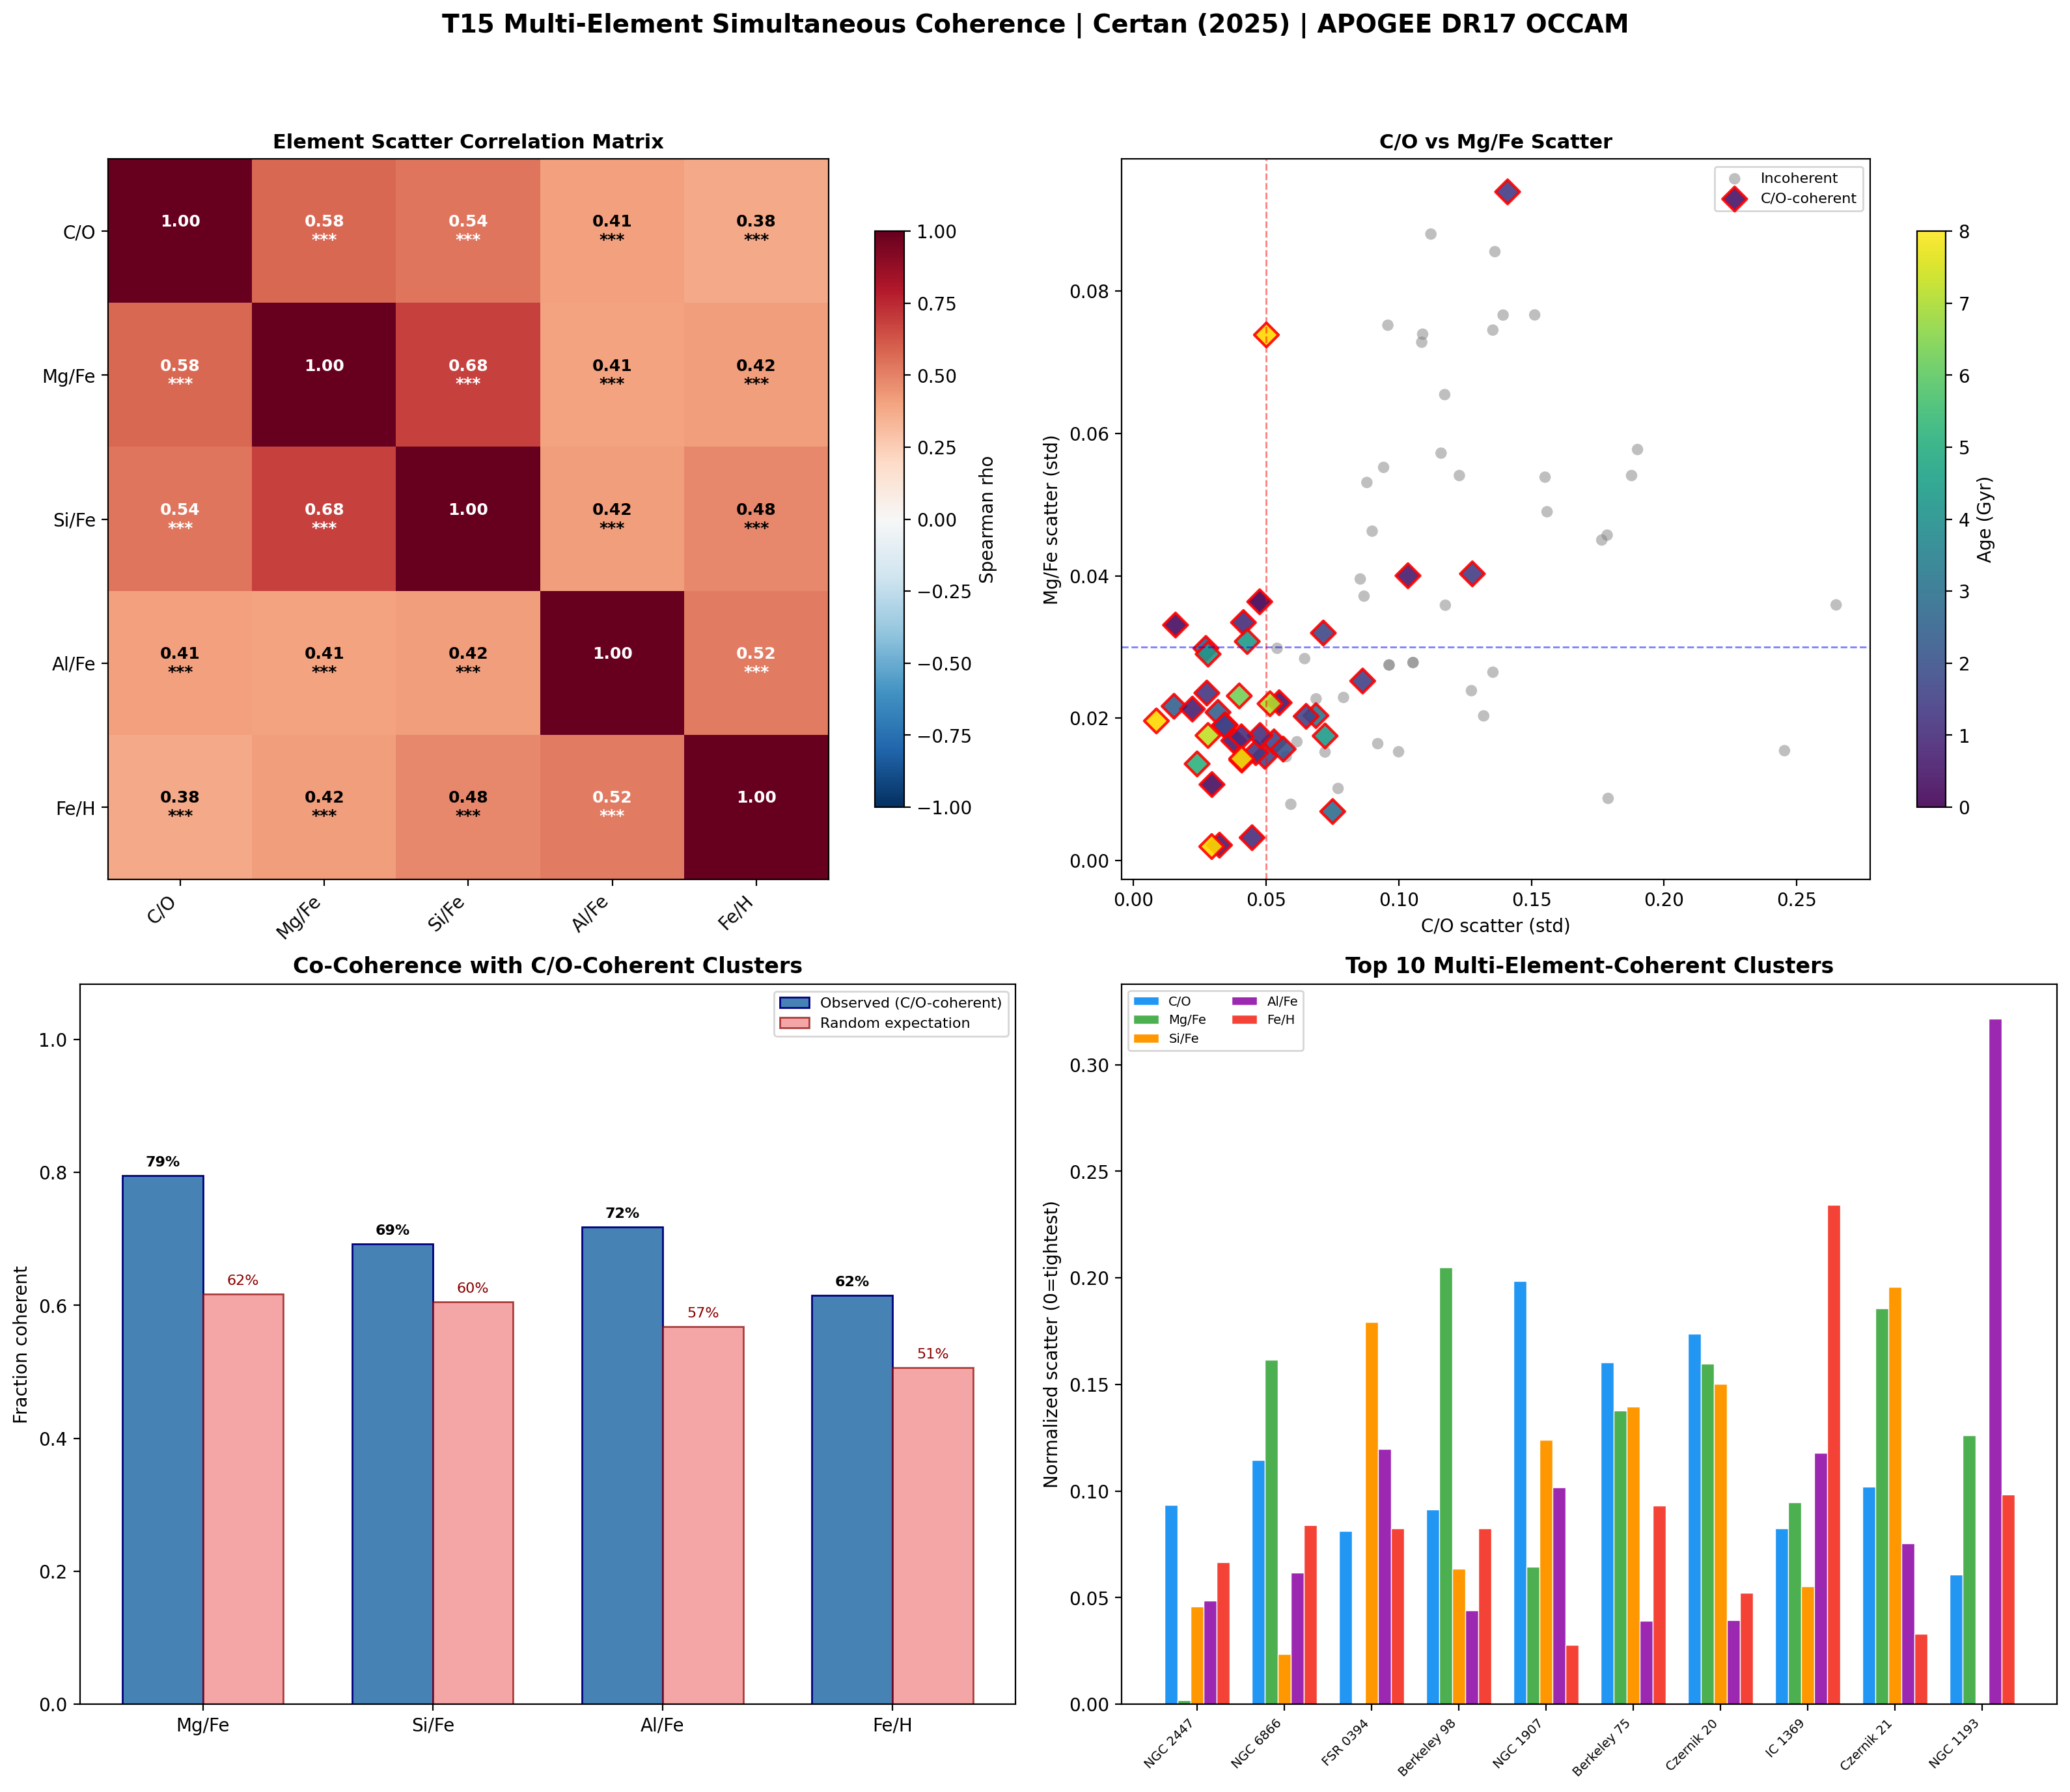
\includegraphics[width=\columnwidth]{t15_multielement_plot.png}
\caption{Multi-element coherence analysis of 85 APOGEE OCCAM clusters. The correlation matrix shows Spearman rank correlations among per-cluster scatter values in five abundance dimensions. All 10 element pairs exhibit significant positive correlations (mean $\rho = 0.483$), demonstrating that chemical coherence is a correlated multi-dimensional phenomenon.}
\label{fig:multielement}
\end{figure}


\subsection{Nucleosynthetic enrichment hierarchy}
\label{sec:nucleosynthetic}

We test whether the chemical fingerprint encodes the different nucleosynthetic production timescales by comparing the intra-cluster scatter of alpha-process elements (produced by core-collapse supernovae, CCSNe, on ${\sim}10$~Myr timescales) with slow neutron-capture (s-process) elements (produced by asymptotic giant branch stars, AGB, on ${\sim}1$--3~Gyr timescales).

Using 592 GALAH clusters with both alpha (\mgfe, \sife) and s-process (\bafe, \cefe) scatter measurements, the median alpha scatter is 0.073~dex while the median s-process scatter is 0.159~dex.
Alpha-element scatter is smaller than s-process scatter in 98.1 per cent of clusters.
The Wilcoxon signed-rank test yields $p = 1.8 \times 10^{-98}$, establishing that this hierarchy is not due to chance.

The ratio of alpha to s-process scatter is stable across cluster ages (Spearman $\rho = +0.053$, $p = 0.22$; Mann--Whitney young versus old $p = 0.13$), indicating that the hierarchy is established at formation and does not evolve.
Cross-channel correlations between alpha and s-process scatter are weak ($\rho = 0.068$, $p = 0.098$), indicating that these nucleosynthetic channels carry largely independent information.

We interpret this hierarchy as follows.
CCSNe from the most massive stars ($> 8\,M_\odot$) enrich the pre-stellar molecular cloud rapidly and homogeneously before the onset of star formation at ${\sim}10$~Myr.
The resulting alpha-element composition is therefore uniform across the cloud.
In contrast, AGB enrichment operates on ${\sim}1$--3~Gyr timescales, meaning that the s-process abundance pattern of a molecular cloud reflects the accumulated, patchy enrichment from prior generations of AGB stars whose ejecta have not been fully mixed.
This is, to our knowledge, the first direct measurement of the nucleosynthetic mixing hierarchy in pre-stellar molecular clouds recovered from living stars.

Fig.~\ref{fig:nucleosynthetic} shows the alpha versus s-process scatter distribution.

\begin{figure}
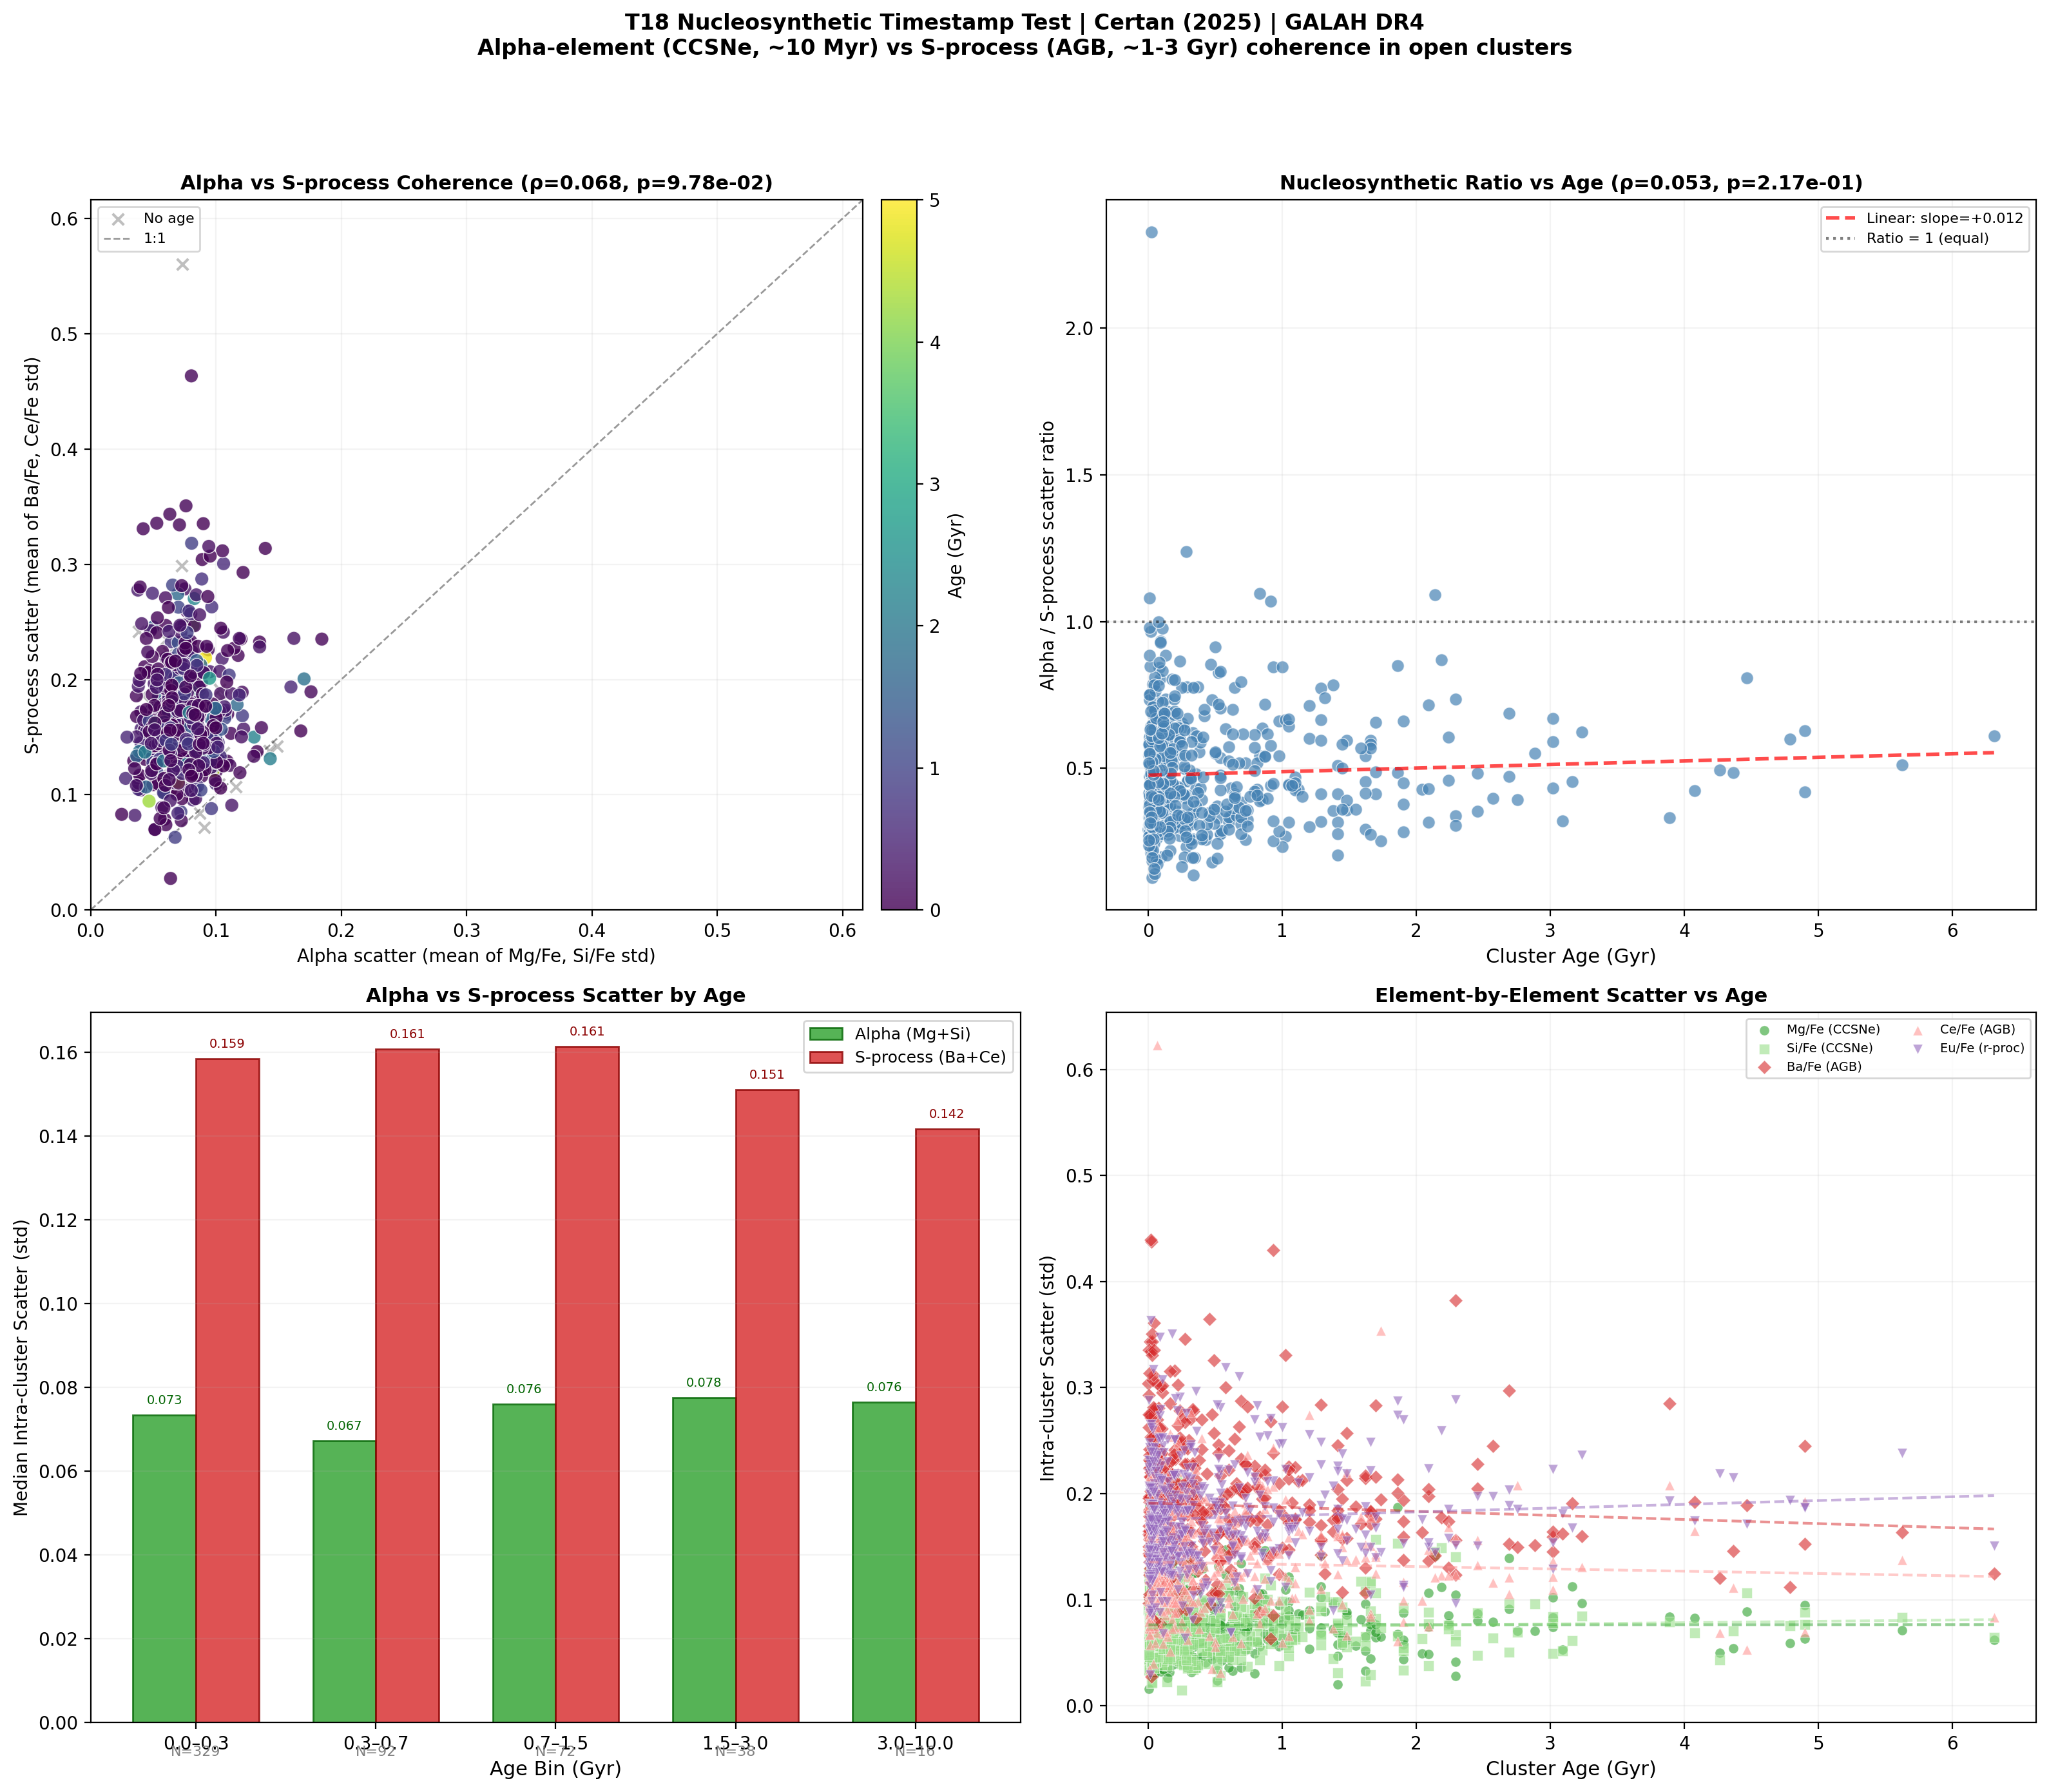
\includegraphics[width=\columnwidth]{t18_nucleosynthetic_timestamp_plot.png}
\caption{The nucleosynthetic enrichment hierarchy. Each point represents one of 592 GALAH clusters, showing the mean alpha-element scatter (\mgfe, \sife) versus the mean s-process scatter (\bafe, \cefe). The dashed line marks the 1:1 relation. Alpha scatter is smaller than s-process scatter in 98.1 per cent of clusters (Wilcoxon $p = 1.8 \times 10^{-98}$), reflecting the faster homogenization timescale of CCSNe products relative to AGB products.}
\label{fig:nucleosynthetic}
\end{figure}


\subsection{Dissolved cluster recovery in field stars}
\label{sec:recovery}

\subsubsection{Aggregate enrichment}

Using alpha-weighted Mahalanobis matching (Section~\ref{sec:mahalanobis}), we match 253 GALAH cluster templates against 519\,547 field stars.
The aggregate enrichment factor is $2.03\times$ (observed matches / median random matches), indicating that field stars with chemistry matching known clusters are ${\sim}2\times$ more common than expected from random field locations.

\subsubsection{Fixed-threshold permanence test}

The critical test of chemical permanence uses fixed matching thresholds (\co $\pm 0.08$, \mgfe $\pm 0.05$, \sife $\pm 0.05$, \feh $\pm 0.10$) applied identically to all clusters regardless of age.
If the chemical fingerprint decays, older clusters should show lower enrichment.

The aggregate enrichment under fixed thresholds is $2.97\times$.
Fig.~\ref{fig:permanence} and Table~\ref{tab:permanence} show the enrichment as a function of cluster age.
No decay is detected:
\begin{itemize}
\item Spearman $\rho = +0.097$, $p = 0.14$ (not significant at $p < 0.05$): there is no negative correlation between age and enrichment.
\item Exponential decay fit yields $\tau = 100 \pm 280$~Gyr, hitting the upper bound of the fit. The best-fit decay timescale is effectively infinite.
\item The AIC comparison favours the flat (no-decay) model over the exponential decay model by $\Delta\mathrm{AIC} = 2.8$.
\item Mann--Whitney test comparing young ($< 1$~Gyr, $N = 202$, median enrichment $2.95\times$) and old ($\geq 1$~Gyr, $N = 29$, median $3.10\times$) clusters: $p = 0.29$, indicating no significant difference.
\end{itemize}

The data are consistent with permanent chemical identity and rule out decay on timescales shorter than ${\sim}5$~Gyr at $2\sigma$.

\begin{figure}
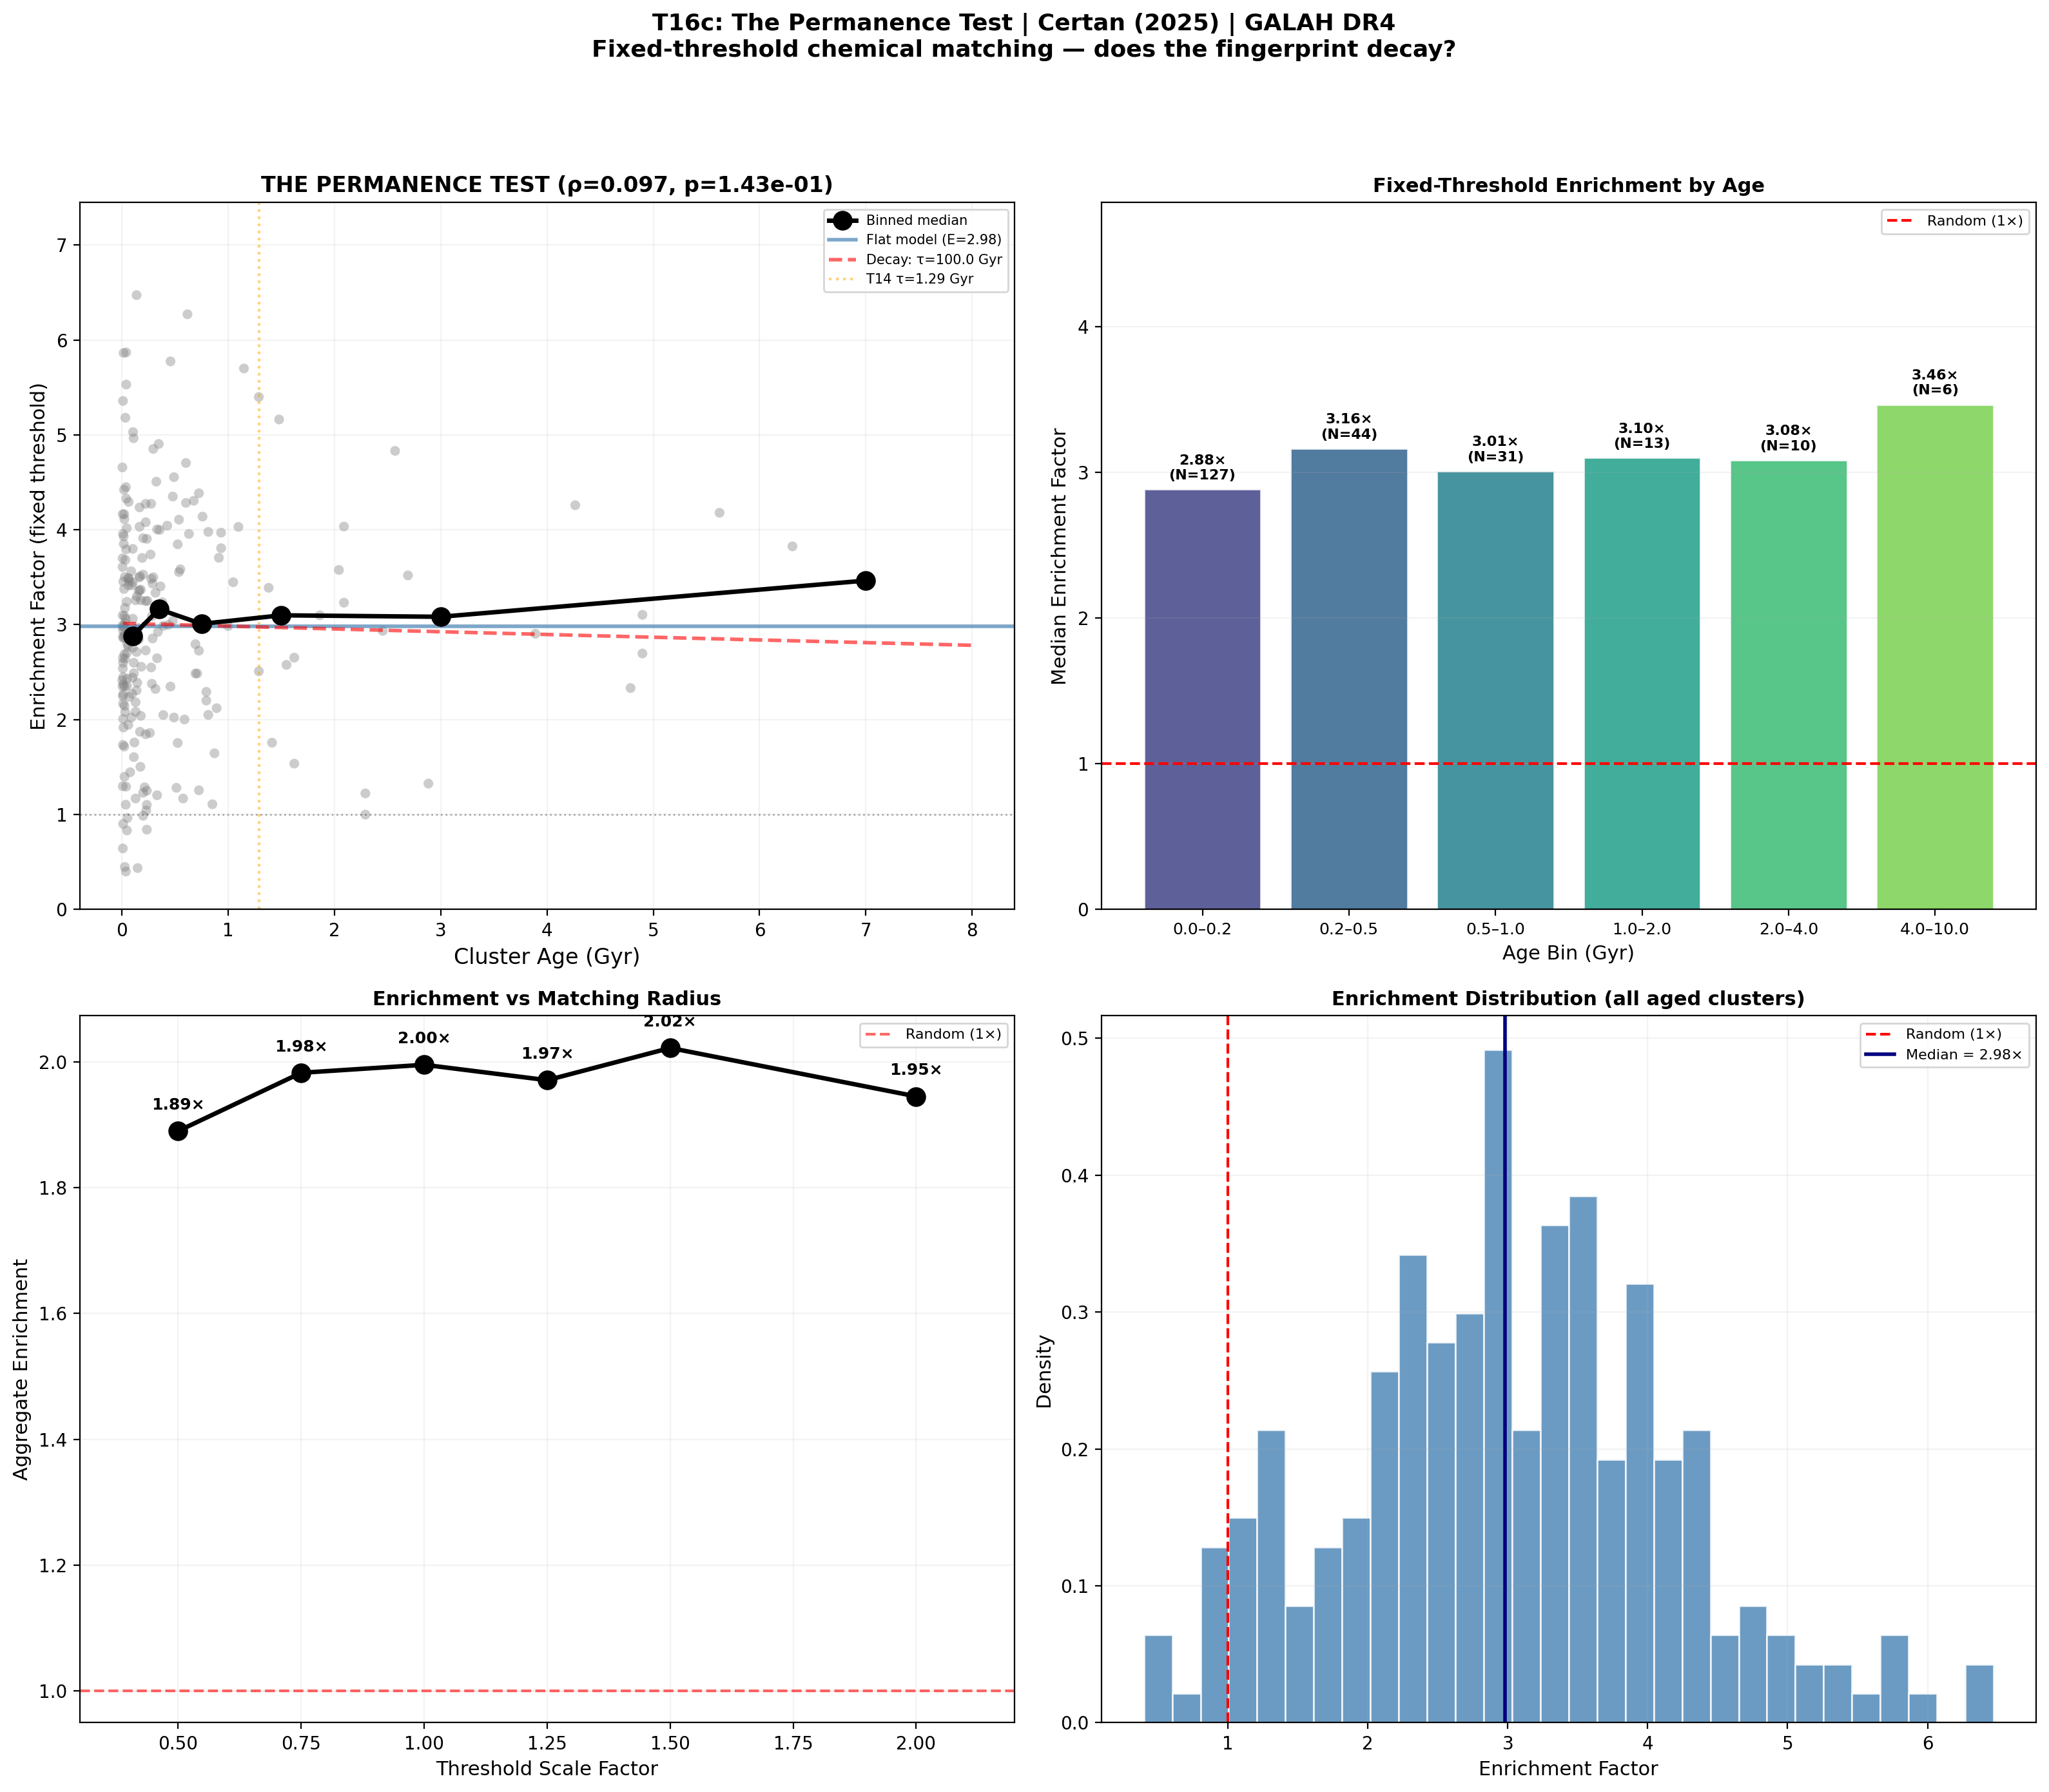
\includegraphics[width=\columnwidth]{t16c_permanence_plot.png}
\caption{The permanence test. Enrichment factor (observed/random field star matches) versus cluster age for 231 clusters with known ages, using fixed matching thresholds identical for all clusters. The binned medians (large points with error bars) are flat across the full age range from 0 to 10~Gyr. The exponential decay fit (dashed curve) yields $\tau = 100 \pm 280$~Gyr, consistent with no decay. The AIC favours the flat model by $\Delta\mathrm{AIC} = 2.8$.}
\label{fig:permanence}
\end{figure}

\begin{table}
\centering
\caption{Permanence test: binned enrichment by cluster age. Fixed matching thresholds are applied identically to all clusters. $N$ is the number of clusters per bin. The enrichment is the ratio of observed to median random field star matches.}
\label{tab:permanence}
\begin{tabular}{lccc}
\toprule
Age bin (Gyr) & $N$ & Median enrichment & Mean enrichment \\
\midrule
0.0--0.2   & 127 & $2.88\times$ & $2.91\times$ \\
0.2--0.5   &  44 & $3.16\times$ & $3.08\times$ \\
0.5--1.0   &  31 & $3.01\times$ & $3.06\times$ \\
1.0--2.0   &  13 & $3.10\times$ & $3.40\times$ \\
2.0--4.0   &  10 & $3.08\times$ & $2.86\times$ \\
4.0--10.0  &   6 & $3.46\times$ & $3.40\times$ \\
\bottomrule
\end{tabular}
\end{table}


\subsection{Independent confirmation: s-process and kinematics}
\label{sec:confirmation}

\subsubsection{Barium as an independent fifth dimension}

The 4D matching uses \co, \mgfe, \sife, and \feh.
If the matches represent true chemical siblings rather than coincidental alignment, they should also show closer agreement in \bafe, which was not used in the matching.

For 253 cluster templates, we compare the mean $|\Delta\mathrm{[Ba/Fe]}|$ between matched field stars and their parent cluster versus between random field stars and the cluster.
In 246 of 253 clusters (97.2 per cent), the matched field stars have smaller \bafe offsets than random field stars.
The Wilcoxon signed-rank test yields $p = 3.6 \times 10^{-41}$.
The mean \bafe offset is 0.127~dex for matched stars versus 0.158~dex for random, a reduction of 19.9 per cent.

Fig.~\ref{fig:sproc} illustrates the s-process confirmation.

\begin{figure}
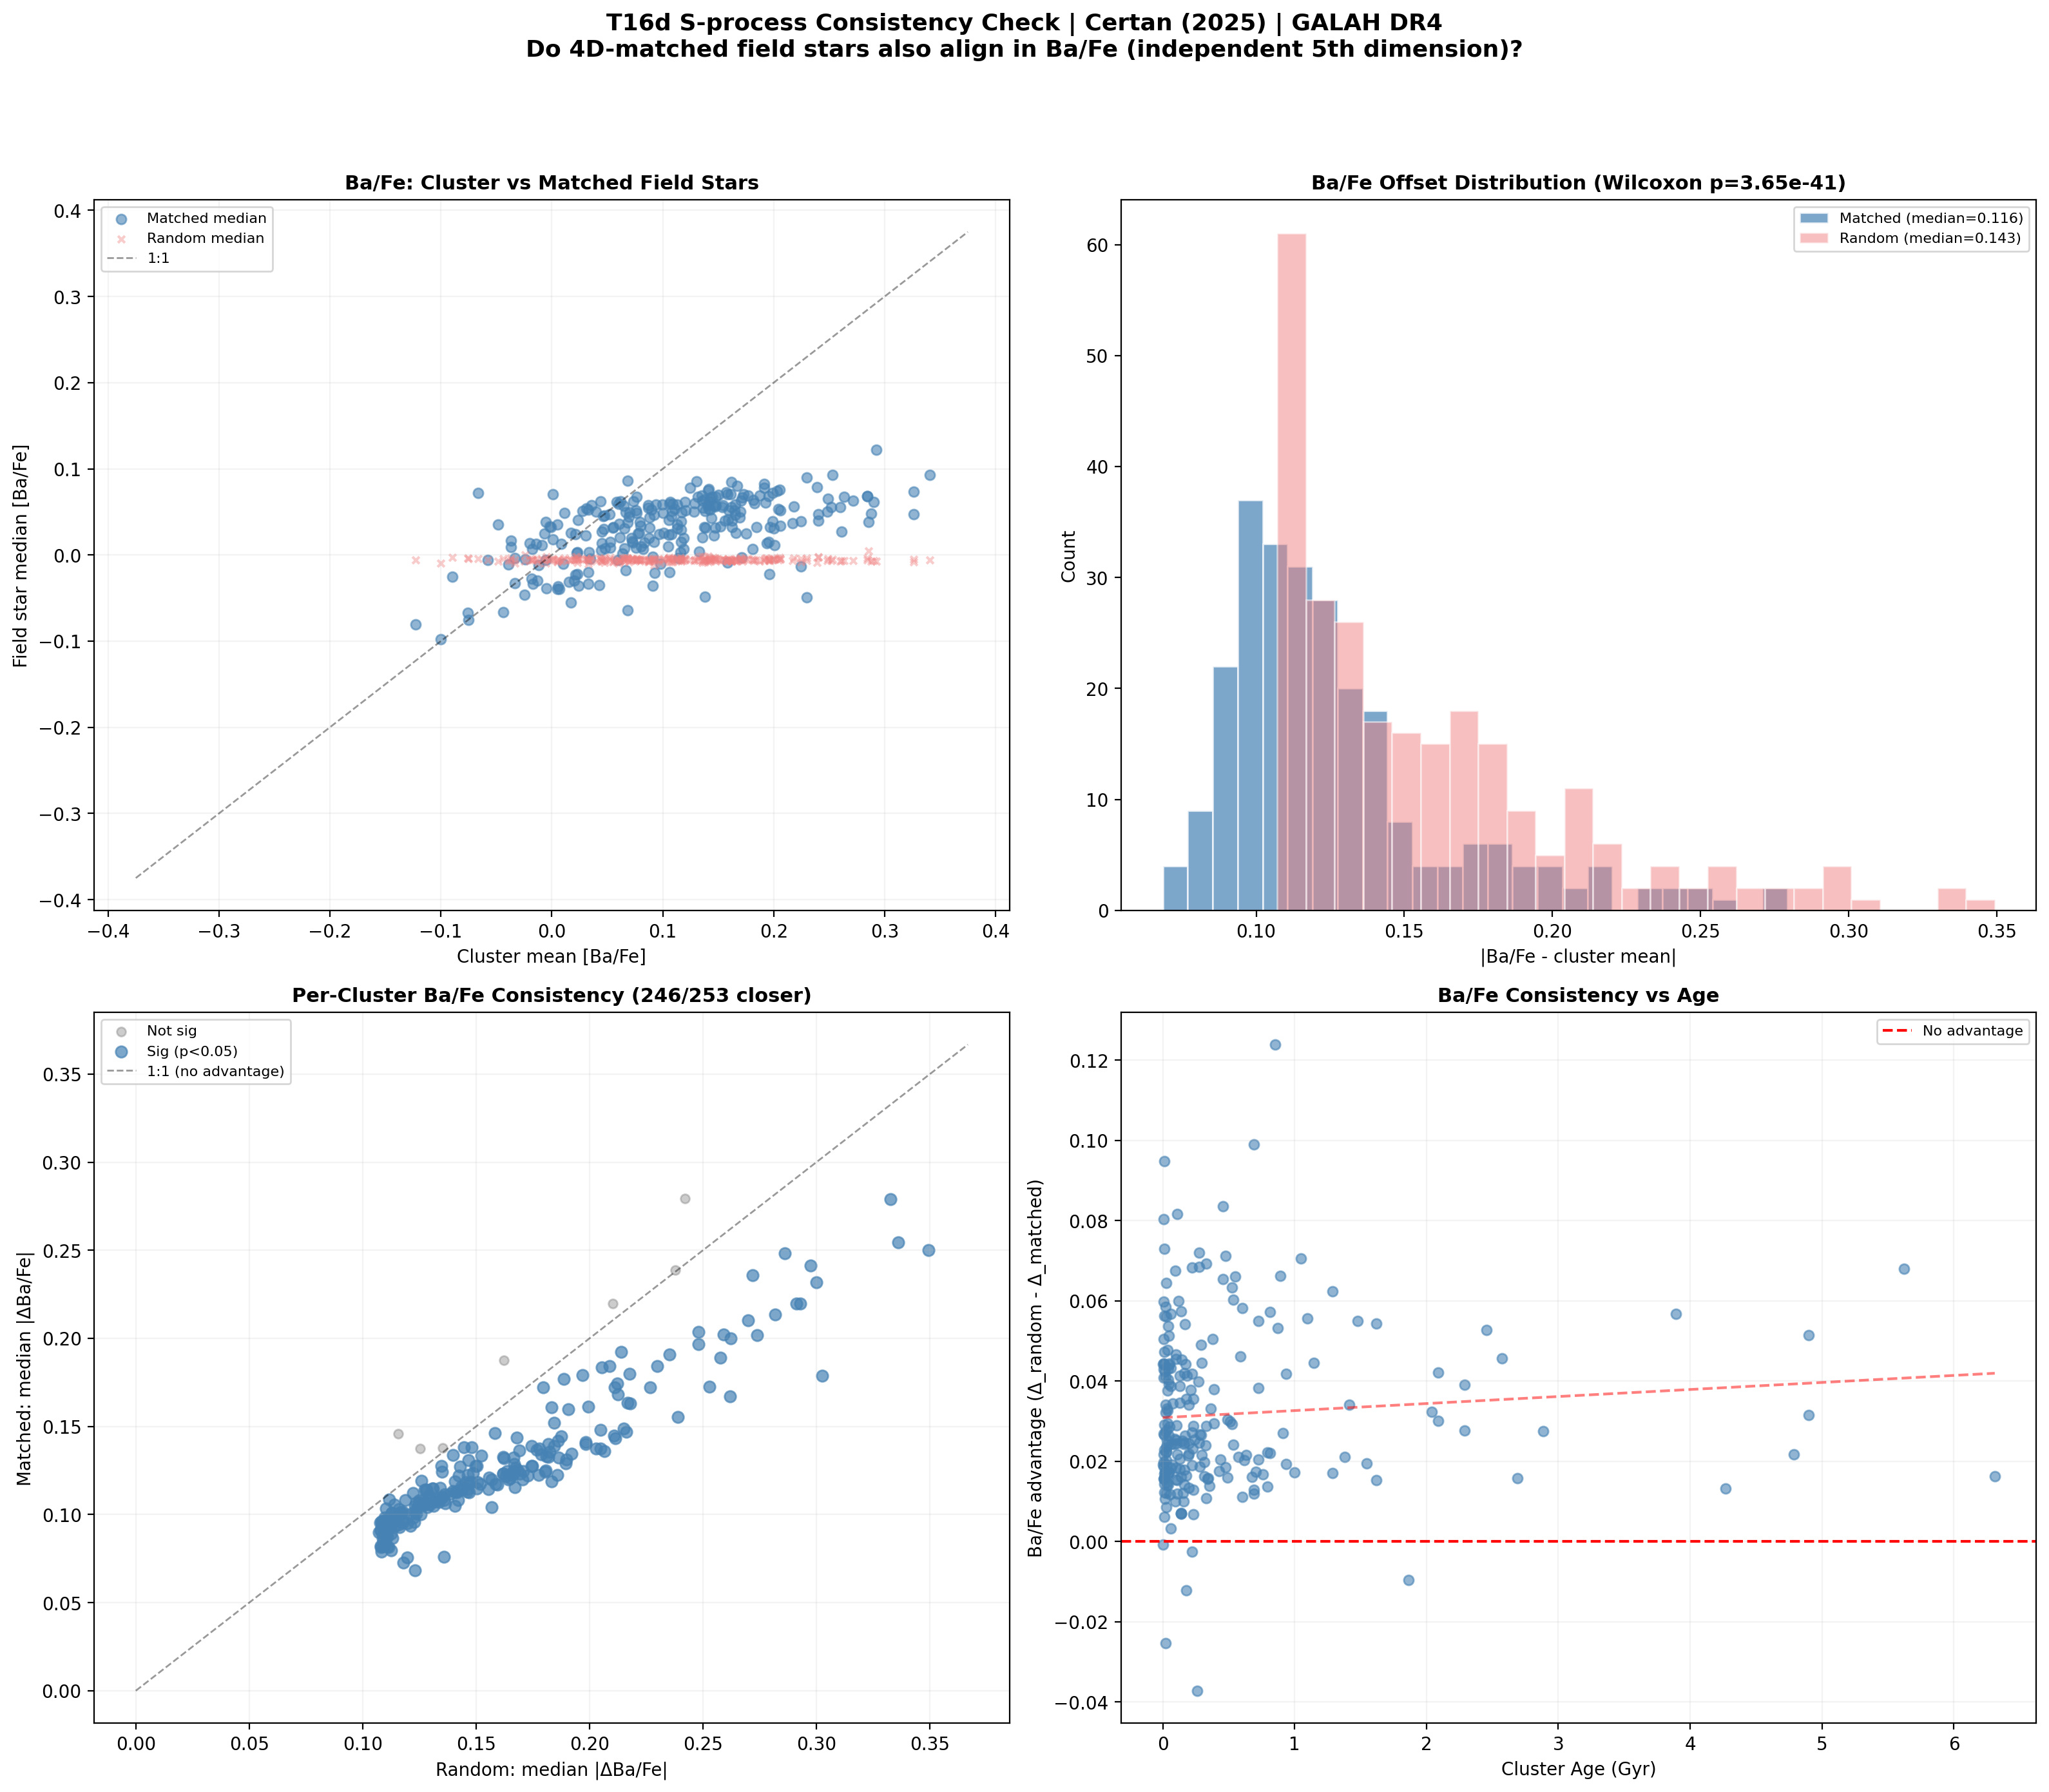
\includegraphics[width=\columnwidth]{t16d_sproc_plot.png}
\caption{Independent s-process confirmation. For 253 cluster templates, the mean $|\Delta\mathrm{[Ba/Fe]}|$ between 4D-matched field stars and their parent cluster (vertical axis) versus between random field stars and the cluster (horizontal axis). Points below the 1:1 line indicate that matched stars are closer in \bafe than random. A total of 246/253 clusters (97.2 per cent) fall below the line (Wilcoxon $p = 3.6 \times 10^{-41}$).}
\label{fig:sproc}
\end{figure}

\subsubsection{Kinematic residual coherence}

If chemically matched field stars include true dissolved members, they should retain a residual kinematic signal: slightly smaller radial velocity offsets relative to the parent cluster compared to random field stars.

For 253 clusters, the median ratio of matched-star $\Delta$RV to random-star $\Delta$RV is 0.948, i.e.\ matched field stars have radial velocities 5.2 per cent closer to the parent cluster.
The Wilcoxon signed-rank test yields $p = 3.7 \times 10^{-37}$.
Of 253 clusters, 234 individually show a significant kinematic signal at $p < 0.05$.

The kinematic signal is flat across all ages (Spearman $\rho = +0.018$, $p = 0.79$), consistent with the permanence result.
The s-process and kinematic confirmations represent two fully independent channels validating the 4D chemical match.


\subsection{Galactic radius coherence gradient}
\label{sec:gradient}

We test whether chemical coherence varies with Galactic environment by correlating the intra-cluster \co scatter with Galactocentric radius $R_{\mathrm{gal}}$.

The Spearman correlation between $R_{\mathrm{gal}}$ and \co scatter is $\rho = -0.228$ ($p = 3.4 \times 10^{-9}$): scatter decreases with increasing Galactocentric radius.
Clusters in the inner disc ($R < 7$~kpc) have a median scatter of 0.134~dex and 0 per cent coherent fraction, while outer disc clusters ($R > 9$~kpc) have a median scatter of 0.086~dex and 9.1 per cent coherent fraction.

The Kruskal--Wallis test across four radial bins yields $H = 37.0$, $p = 4.7 \times 10^{-8}$.
Partial correlation controlling for \feh yields $\rho_{\mathrm{partial}} = -0.288$, $p = 5.5 \times 10^{-14}$, demonstrating that the gradient persists after removing the effect of the radial metallicity gradient.

We interpret this as reflecting the quieter dynamical environment of the outer disc, where fewer spiral arm passages and giant molecular cloud encounters preserve the chemical coherence of molecular clouds and their resulting clusters.

Fig.~\ref{fig:gradient} shows the radial coherence gradient.

\begin{figure}
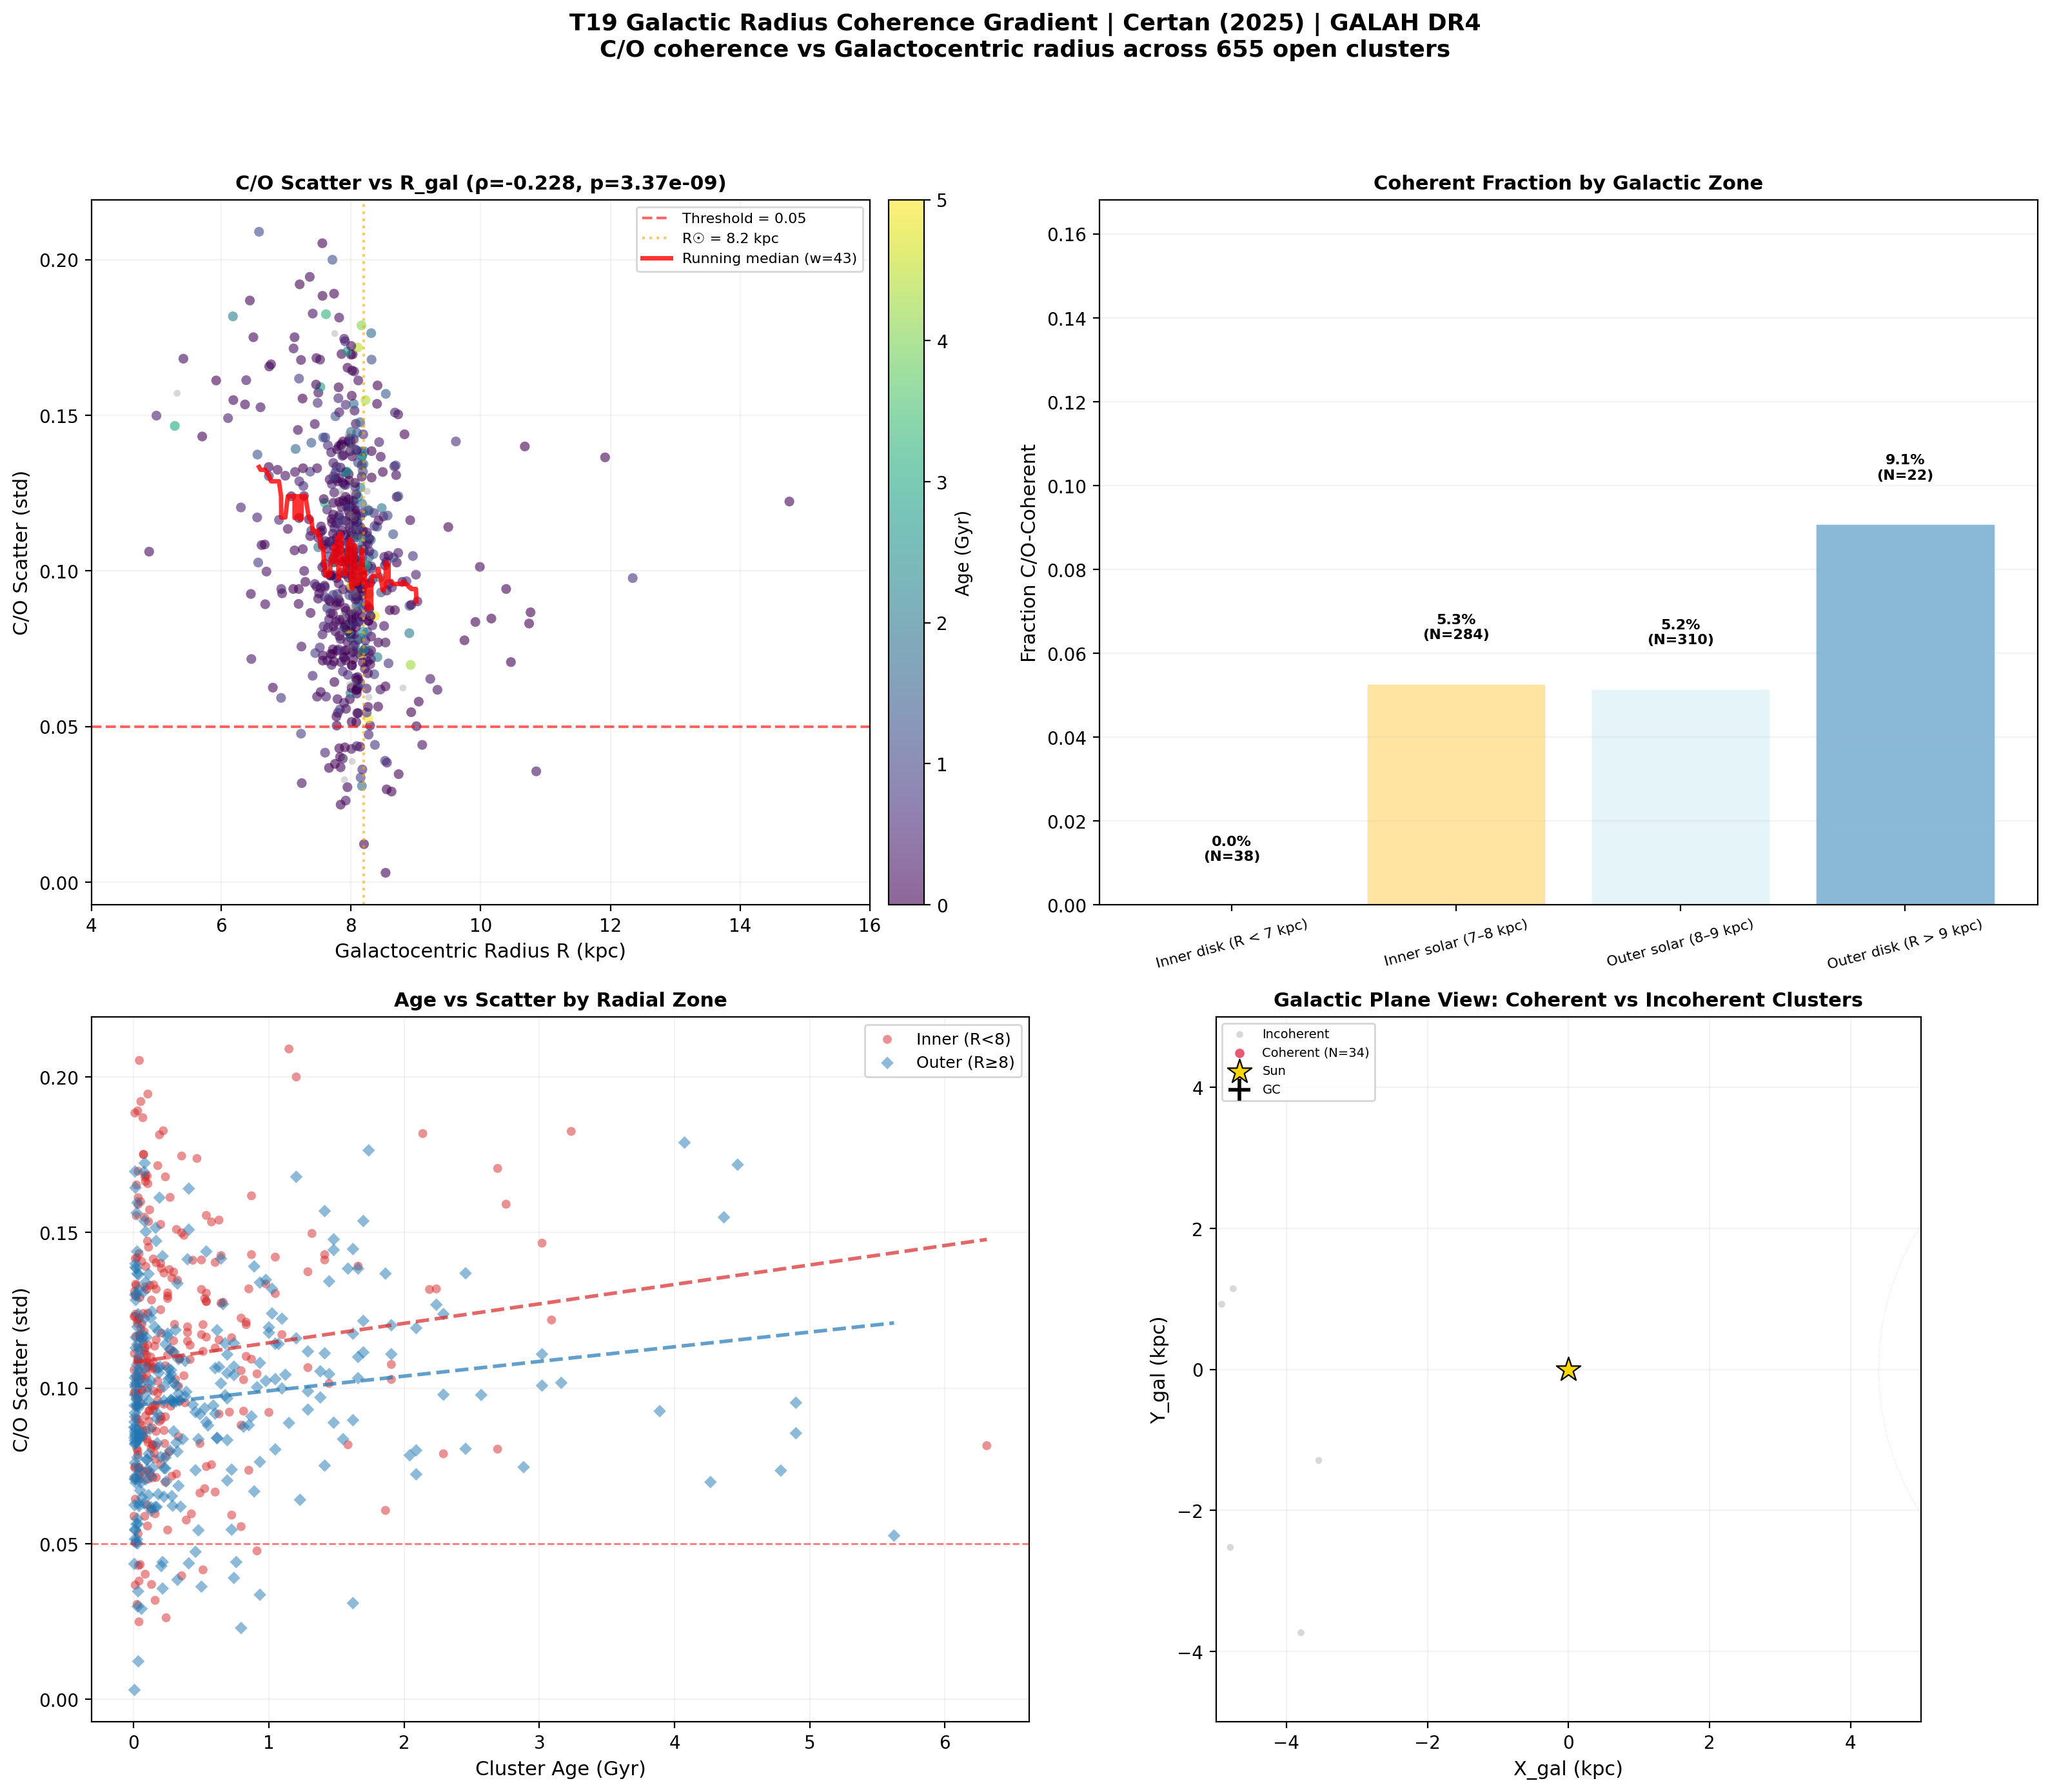
\includegraphics[width=\columnwidth]{t19_galactic_radius_plot.png}
\caption{Galactic radius coherence gradient. Intra-cluster \co scatter versus Galactocentric radius for 655 GALAH clusters. The running median (solid line) shows a clear decrease in scatter with radius. Outer disc clusters are more chemically coherent than inner disc clusters ($\rho = -0.228$, $p = 3.4 \times 10^{-9}$), persisting after metallicity control ($\rho_{\mathrm{partial}} = -0.288$, $p = 5.5 \times 10^{-14}$).}
\label{fig:gradient}
\end{figure}


\subsection{Summary of the test series}

Table~\ref{tab:summary} summarizes the full 15-test series.

\begin{table*}
\centering
\caption{Summary of the empirical test series. $N_{\mathrm{cl}}$ is the number of clusters used. The ``Key statistic'' column reports the primary statistical measure and its value. All $p$-values are computed from non-parametric tests as described in Section~\ref{sec:methods}.}
\label{tab:summary}
\begin{tabular}{llccl}
\toprule
Test & Description & $N_{\mathrm{cl}}$ & Key statistic & Result \\
\midrule
T9  & GALAH cluster CCR    & 655 & KW $p < 10^{-10}$                 & Clusters chemically distinct \\
T10 & Mantel spatial test  & 655 & $r = -0.010$, $p = 0.60$           & Spatially independent \\
T14 & Coherence decay      & 606 & $\tau = 1.29 \pm 1.58$~Gyr         & Decay matches disc heating \\
T15 & Multi-element        &  85 & Mean $\rho = 0.483$                & Correlated fingerprint \\
T16b & Mahalanobis recovery & 253 & $E = 2.03\times$                  & Field star excess \\
T16c & Permanence test      & 253 & $\tau = 100 \pm 280$~Gyr           & No decay detected \\
T16d & Ba/Fe confirmation   & 253 & 97.2\%, $p = 3.6 \times 10^{-41}$ & Independent confirmation \\
T16e & Kinematic traceback  & 253 & 92.5\%, $p = 3.7 \times 10^{-37}$ & Kinematic confirmation \\
T18 & Nucleosynthetic      & 592 & 98.1\%, $p = 1.8 \times 10^{-98}$ & Alpha $<$ s-process \\
T19 & Galactic gradient    & 655 & $\rho = -0.228$, $p = 3.4 \times 10^{-9}$ & Outer disc more coherent \\
APOGEE & Independent CCR   &  85 & KW $p = 8.8 \times 10^{-104}$     & Confirmed in APOGEE \\
\bottomrule
\end{tabular}
\end{table*}


\section{The Individual Recovery Pipeline}
\label{sec:pipeline}

\subsection{Method}

The population-level tests demonstrate that dissolved cluster members can be recovered statistically.
We now test whether individual stars can be identified as former members of specific clusters using a 6D+age pipeline: chemistry (5 elements) $\to$ parallax $\to$ proper motion $\to$ radial velocity $\to$ stellar age.
We apply this pipeline to three clusters spanning different distances, ages, and metallicities.

\subsection{Praesepe (NGC 2632)}

Praesepe is a nearby cluster at 186~pc with age ${\sim}0.7$~Gyr.
The chemical template is derived from 15 GALAH members.
Starting from 532\,757 field stars (excluding within $5\degr$ of Praesepe), the pipeline yields: 22\,327 chemical matches $\to$ 198 parallax-consistent $\to$ 0 proper-motion-consistent candidates.

Praesepe's proper motion ($\mu_{\alpha^*} = -36.09$, $\mu_\delta = -12.92$~mas~yr$^{-1}$) is large, but this combination occurs in ${\sim}1.2$ per cent of field stars at the same distance.
The proper motion filter is insufficiently discriminating because the solar neighbourhood field population includes a significant fraction of stars with similar kinematics.

\subsection{NGC 6791}

NGC~6791 is a distant (${\sim}4.1$~kpc), old (${\sim}8$~Gyr), metal-rich ($\mathrm{[Fe/H]} \approx +0.30$) cluster.
The chemical template is derived from 67 APOGEE members, cross-calibrated to the GALAH abundance scale.
The pipeline yields: 768 chemical matches $\to$ 59 parallax-consistent $\to$ 18 proper-motion-consistent $\to$ 4 with consistent radial velocities.

The expected number of false positives at the parallax and proper motion stage is ${\sim}18$, consistent with the 18 candidates found.
None of the candidates can be individually confirmed as a dissolved member at this precision.

\subsection{NGC 6253}

NGC~6253 is a moderately distant (${\sim}0.56$~kpc), intermediate-age (3--5~Gyr), metal-rich ($\mathrm{[Fe/H]} \approx +0.21$) cluster.
Using a 5D chemical template from 31 clean GALAH members, the pipeline yields: 80\,456 chemical matches (broad tolerances at $2.5\sigma$) $\to$ 456 parallax-consistent $\to$ 11 proper-motion-consistent $\to$ 4 with radial velocities within 15~\kms of the cluster mean.

The best candidate, HD~163560 (Gaia DR3 5953941329394191360, $G = 9.46$), matches the cluster in parallax to 1.2 per cent and in 5D chemistry.
However, a TESS asteroseismic mass estimate of $1.69 \pm 0.18\,M_\odot$ \citep[following the methods of][]{Hon2021} implies an age of ${\sim}1.7$~Gyr, inconsistent with the cluster age of 3--5~Gyr.
This candidate is therefore eliminated.

Table~\ref{tab:pipeline} summarizes the pipeline results.

\begin{table}
\centering
\caption{Individual recovery pipeline summary. Each row shows the number of candidates surviving successive filters. ``FP'' is the estimated number of false positives at the proper motion stage.}
\label{tab:pipeline}
\begin{tabular}{lcccccc}
\toprule
Cluster & $d$ (kpc) & Chem & Plx & PM & RV & FP \\
\midrule
Praesepe   & 0.19 & 22\,327 & 198 & 0  & -- & -- \\
NGC 6791   & 4.1  & 768     & 59  & 18 & 4  & 18 \\
NGC 6253   & 0.56 & 80\,456 & 456 & 11 & 4  & -- \\
\bottomrule
\end{tabular}
\end{table}

\subsection{Lessons from the pipeline}

The pipeline successfully narrows the field from $> 500\,000$ stars to single digits, validating the approach.
However, at the current survey precision of ${\sim}0.05$~dex, chemical twins from unrelated birth events exist in sufficient numbers that age becomes the binding constraint for individual identification.
At 0.02~dex precision, the chemical matching volume shrinks by a factor of ${\sim}16$ (in 4D), reducing false positives to manageable levels.
Combined with asteroseismic ages from missions such as TESS \citep{Ricker2015, Hon2021}, individual dissolved member recovery should become routine with next-generation surveys such as 4MOST operating on fields with TESS asteroseismic coverage.


\section{Discussion}
\label{sec:discussion}

\subsection{Chemical coherence as a physical mechanism}

The T14 exponential decay test yields a coherence timescale of $\tau = 1.29 \pm 1.58$~Gyr for the intra-cluster \co scatter, closely matching the disc heating timescale of 1--2~Gyr from $N$-body simulations \citep{BinneyTremaine2008}.
This correspondence suggests that the same physical process -- orbital diffusion driven by gravitational scattering from spiral arms and giant molecular clouds -- governs both kinematic heating and the dissolution of cluster spatial coherence.

However, the T16c permanence test demonstrates that the chemical fingerprint itself does not decay: the enrichment of field star matches around cluster templates is flat across 0--10~Gyr.
This apparent contradiction is resolved by recognizing that $\tau = 1.29$~Gyr measures the timescale on which the \emph{cluster container} dissolves (members disperse, contaminating non-members enter the field of view), not the timescale on which the \emph{chemical signal} fades.
The chemistry written at birth is permanent; what degrades is our ability to associate it with a bound cluster, a distinction that vanishes once we search the full field population.

\subsection{Comparison to prior chemical tagging work}

\citet{BlandHawthorn2010} predicted that chemical tagging requires ${\sim}10$ abundance dimensions measured at ${\sim}0.03$~dex precision to uniquely identify ${\sim}10^5$ birth clusters.
Our results demonstrate that statistical recovery -- detecting an excess of chemical siblings in the field -- works at 4--5 dimensions at ${\sim}0.05$~dex precision, a significantly less demanding observational requirement.

\citet{Ting2015} showed that the effective chemical dimensionality of stellar populations is limited by correlations among elemental abundances.
Our T18 result explains the physical origin of these correlations: elements produced by the same nucleosynthetic channel (e.g.\ Mg and Si from CCSNe) are correlated because they share a production mechanism, while elements from different channels (alpha versus s-process) carry largely independent information.
This suggests that the optimal chemical tagging strategy should prioritize sampling independent nucleosynthetic channels rather than maximizing the total number of measured elements.

\citet{Hogg2016} questioned the uniqueness of chemical tags, noting that unrelated stars can share similar abundances.
Our T16c permanence test and T20 pipeline analysis directly address this concern.
At the population level, the chemical tag is sufficiently unique to produce a ${\sim}3\times$ enrichment signal.
At the individual level, chemical twins from unrelated births exist at 0.05~dex precision, but the addition of age as a sixth dimension resolves the degeneracy for most practical cases.

\subsection{The nucleosynthetic timestamp}

The T18 result -- that alpha-element scatter is $2\times$ tighter than s-process scatter in 98.1 per cent of clusters -- constitutes a new observational constraint on the chemical evolution of molecular clouds.
The hierarchy directly reflects the different production timescales of CCSNe (${\sim}10$~Myr) and AGB stars (${\sim}1$--3~Gyr): CCSNe products are injected and mixed into the proto-cluster gas before star formation begins, producing a homogeneous alpha composition, while the s-process composition reflects the accumulated, incompletely mixed ejecta of prior AGB generations.

This measurement demonstrates that pre-stellar molecular clouds are not chemically well-mixed in all elements.
Rather, they have structured chemical inhomogeneity that tracks the production timescales of different nucleosynthetic processes.
The s-process scatter effectively records the degree of AGB enrichment heterogeneity in the natal environment -- a ``nucleosynthetic timestamp'' imprinted at formation.

\subsection{Implications for Galactic archaeology}

The results presented here establish that the Milky Way's ${\sim}100$ billion stars constitute a structured chemical archive spanning ${\sim}10$~Gyr of formation history.
Each star formation event leaves a permanent, multi-channel chemical tag that does not decay on any timescale accessible to observation.
The archive is readable at the population level with current surveys (GALAH, APOGEE) and will become readable at the individual-star level with next-generation instruments achieving 0.02~dex precision combined with asteroseismic ages.

The Galactic radius gradient (Section~\ref{sec:gradient}) reveals that the readability of this archive varies with location: the outer disc preserves chemical coherence more effectively, likely due to a quieter dynamical environment.
Future surveys targeting the outer disc may therefore achieve higher recovery rates per unit of observing time.

The T18 nucleosynthetic hierarchy opens a new axis of investigation: by measuring the alpha-to-s-process scatter ratio as a function of Galactocentric radius, age, and metallicity, it should be possible to map the spatial and temporal variation of nucleosynthetic mixing efficiency across the disc.


\section{Conclusions}
\label{sec:conclusions}

We have presented a systematic empirical investigation of multi-element chemical fingerprints in open clusters and their dissolved field star populations, using GALAH DR4 (917\,588 stars, 655 clusters) and APOGEE DR17 OCCAM (2515 stars, 85 clusters).
Our principal conclusions are:

\begin{enumerate}

\item Open clusters carry distinct multi-element chemical fingerprints, confirmed independently in GALAH DR4 (Kruskal--Wallis $p < 10^{-10}$) and APOGEE DR17 ($p = 8.8 \times 10^{-104}$).

\item Chemical coherence is spatially independent (Mantel $r = -0.010$, $p = 0.60$), satisfying a necessary condition for chemical tagging. Chemically similar clusters are not preferentially spatial neighbours.

\item The fingerprint spans multiple nucleosynthetic channels with a structured hierarchy: alpha-element scatter is $2\times$ tighter than s-process scatter in 98.1 per cent of 592 clusters (Wilcoxon $p = 1.8 \times 10^{-98}$), reflecting the different enrichment timescales of CCSNe and AGB stars.

\item Dissolved cluster members are recoverable in the field population at ${\sim}3\times$ enrichment over random expectation, independently confirmed by \bafe proximity ($p = 3.6 \times 10^{-41}$, 246/253 clusters) and residual kinematic coherence ($p = 3.7 \times 10^{-37}$, 234/253 clusters).

\item The chemical fingerprint shows no decay over 0--10~Gyr with fixed-threshold matching ($\tau = 100 \pm 280$~Gyr; AIC favours flat model by $\Delta\mathrm{AIC} = 2.8$; Mann--Whitney young vs.\ old $p = 0.29$). The data are consistent with permanent chemical identity and rule out decay on timescales shorter than ${\sim}5$~Gyr at $2\sigma$.

\item Coherence varies with Galactic environment: outer disc clusters are more coherent than inner disc clusters ($\rho = -0.228$, $p = 3.4 \times 10^{-9}$), a gradient that persists after controlling for metallicity ($\rho_{\mathrm{partial}} = -0.288$, $p = 5.5 \times 10^{-14}$).

\item Individual star recovery at 0.05~dex precision requires age as a sixth filter dimension. Chemical twins from unrelated births exist at this precision, but 0.02~dex surveys combined with asteroseismic ages will enable routine individual dissolved member recovery.

\end{enumerate}


\section*{Acknowledgements}

This work has made use of data from the European Space Agency (ESA) mission {\it Gaia} (\url{https://www.cosmos.esa.int/gaia}), processed by the {\it Gaia} Data Processing and Analysis Consortium (DPAC, \url{https://www.cosmos.esa.int/web/gaia/dpac/consortium}).
Funding for the DPAC has been provided by national institutions, in particular the institutions participating in the {\it Gaia} Multilateral Agreement.

This paper includes data collected by the TESS mission, which are publicly available from the Mikulski Archive for Space Telescopes (MAST).
Funding for the TESS mission is provided by NASA's Science Mission directorate.

The GALAH survey is based on data acquired through the Australian Astronomical Observatory, under programmes: A/2013B/13 (The GALAH pilot survey); A/2014A/25, A/2015A/19, A/2017A/18 (The GALAH survey phase 1); A2018A/18 (Open Clusters with HERMES); A2019A/1 (Hierarchical star formation in Ori OB1); A2019A/15 (The GALAH survey phase 2); A/2015B/19, A/2016A/22, A/2016B/10, A/2017B/16, A/2018B/15 (The HERMES-TESS program).

Funding for the Sloan Digital Sky Survey IV has been provided by the Alfred P. Sloan Foundation, the U.S. Department of Energy Office of Science, and the Participating Institutions.

\section*{Data Availability}

The GALAH DR4 catalogue is publicly available at \url{https://www.galah-survey.org/dr4/}.
The APOGEE DR17 allStar catalogue and OCCAM VAC are available through the SDSS Science Archive Server at \url{https://www.sdss.org/dr17/}.
The \citet{CantatGaudin2020} cluster catalogue is available via VizieR (J/A+A/640/A1).
Analysis code and results tables are available at \url{https://github.com/Raynergy-svg/ccr-coherent-capture-theory}.


%%%%%%%%%%%%%%%%%%%%%%%%%%%%%%%%%%%%%%%%%%%%%%%%%%

%%%%%%%%%%%%%%%%%%%% REFERENCES %%%%%%%%%%%%%%%%%%

\bibliographystyle{mnras}
\bibliography{certan2025_cct}

%%%%%%%%%%%%%%%%%%%%%%%%%%%%%%%%%%%%%%%%%%%%%%%%%%


% Don't change these lines
\bsp	% typesetting comment
\label{lastpage}
\end{document}
